%%%%%%%%%%%%%%%%%%%%%%%%%%%%%%%%%%%%%%
% LaTeX poster template
% Created by Nathaniel Johnston
% August 2009
% http://www.nathanieljohnston.com/2009/08/latex-poster-template/
%%%%%%%%%%%%%%%%%%%%%%%%%%%%%%%%%%%%%%

\documentclass[final]{beamer}
\usepackage[scale=1.24]{beamerposter}
\usepackage{graphicx}			% allows us to import images
\usepackage{anyfontsize}

%-----------------------------------------------------------
% Define the column width and poster size
% To set effective sepwid, onecolwid and twocolwid values, first choose how many columns you want and how much separation you want between columns
% The separation I chose is 0.024 and I want 4 columns
% Then set onecolwid to be (1-(4+1)*0.024)/4 = 0.22
% Set twocolwid to be 2*onecolwid + sepwid = 0.464
%-----------------------------------------------------------

\newlength{\sepwid}
\newlength{\onecolwid}
\newlength{\twocolwid}
\newlength{\threecolwid}
\setlength{\paperwidth}{40in}
\setlength{\paperheight}{34in}
\setlength{\sepwid}{0.024\paperwidth}
\setlength{\onecolwid}{0.22\paperwidth}
\setlength{\twocolwid}{0.464\paperwidth}
\setlength{\threecolwid}{0.708\paperwidth}
\setlength{\topmargin}{-0.5in}
\usepackage[]{moresize}
\usetheme{confposter}
\usepackage{exscale}

%-----------------------------------------------------------
% The next part fixes a problem with figure numbering. Thanks Nishan!
% When including a figure in your poster, be sure that the commands are typed in the following order:
% \begin{figure}
% \includegraphics[...]{...}
% \caption{...}
% \end{figure}
% That is, put the \caption after the \includegraphics
%-----------------------------------------------------------

\usecaptiontemplate{
\small
\structure{\insertcaptionname~\insertcaptionnumber:}
\insertcaption}

%-----------------------------------------------------------
% Define colours (see beamerthemeconfposter.sty to change these colour definitions)
%-----------------------------------------------------------

\setbeamercolor{block title}{fg=ngreen,bg=white}
\setbeamercolor{block body}{fg=black,bg=white}
\setbeamercolor{block alerted title}{fg=white,bg=dblue!70}
\setbeamercolor{block alerted body}{fg=black,bg=dblue!10}

%-----------------------------------------------------------
% Name and authors of poster/paper/research
%-----------------------------------------------------------

\title{{\fontsize{111}{111}\selectfont Near-inertial waves} \textit{extract energy}
{\fontsize{75}{75}\selectfont from}\\ \hskip2.5cm {\fontsize{75}{75}\selectfont barotropic}
        {\fontsize{111}{111}\selectfont quasi-geostrophic flow} }
\author{\textbf{Cesar B. Rocha} and Gregory L. Wagner and William R. Young}
\institute{\hskip1.25cm crocha\textbf{@ucsd}.edu\hskip2.5cm
           \hskip3.75cm glwagner\textbf{@mit}.edu \hskip2.5cm
           \hskip2.5cm wryoung\textbf{@ucsd}.edu \hskip2.5cm
          }

% adds art to title box
           \setbeamertemplate{headline}{
            \leavevmode
            \begin{columns}
              \begin{column}{.6\linewidth}
               \vskip1cm
               \hskip2.5cm
               \usebeamercolor{title in headline}{\color{jblue}\Huge{\textbf{\inserttitle}}\\[0.5ex]}
               \hskip2.5cm
               \usebeamercolor{author in headline}{\color{fg}\Large{\insertauthor}\\[1ex]}
               \hskip2.5cm
               \usebeamercolor{institute in headline}{\color{fg}\large{\insertinstitute}\\[1ex]}
               \vskip1cm
              \end{column}
              \begin{column}{.4\linewidth}
                \hspace{-4.em}
                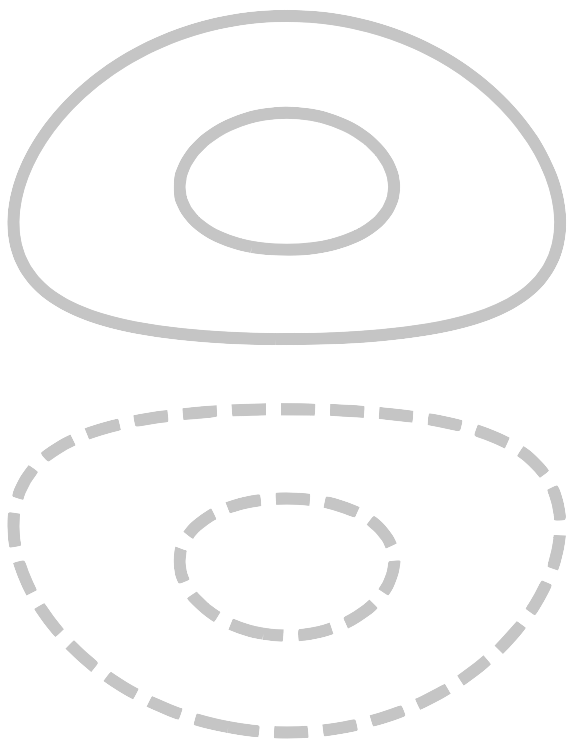
\includegraphics[width=0.2\linewidth]{figs/dipole2art_1.png}\hspace{.5em}
                %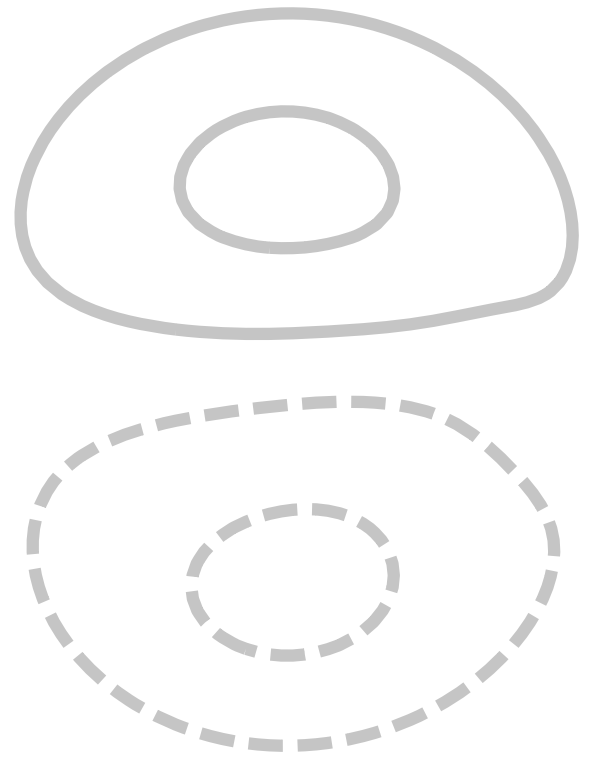
\includegraphics[width=0.2\linewidth]{figs/dipole2art_2.png}\hspace{1.5em}
               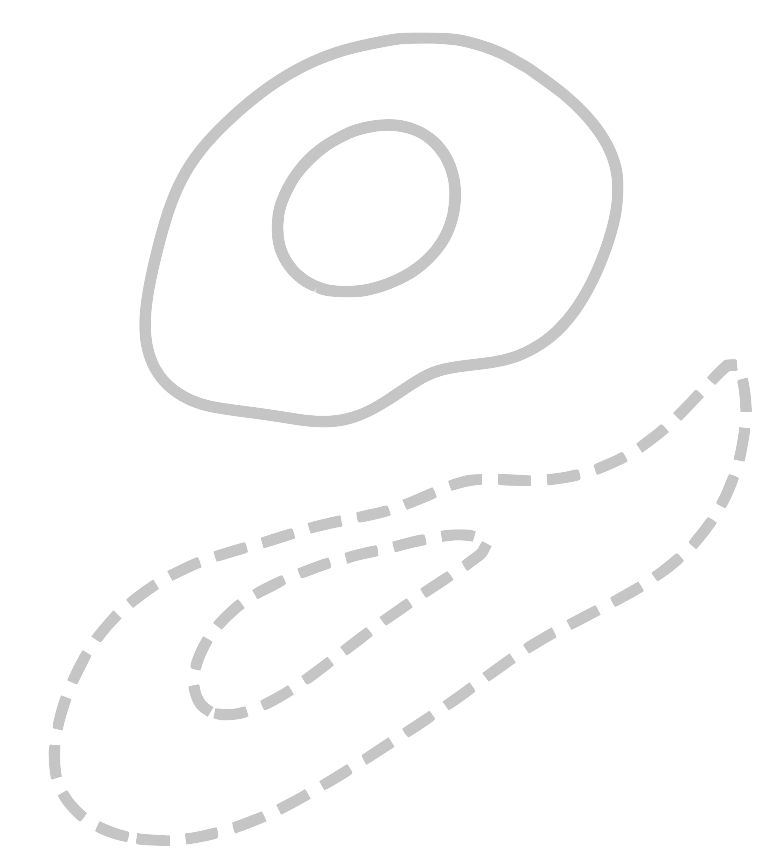
\includegraphics[width=0.25\linewidth]{figs/dipole2art_3.png}\hspace{-6.em}
               
\includegraphics[width=0.315\linewidth]{figs/dipole2art_4.png}
              \end{column}
              \vspace{1cm}
             \end{columns}
            \vspace{0.5in}
            \hspace{0.5in}\begin{beamercolorbox}[wd=39in,colsep=0.15cm]{cboxb}\end{beamercolorbox}

            \vspace{0.1in}
           }
           \newcommand{\defn}{\ensuremath{\stackrel{\mathrm{def}}{=}}}


%-----------------------------------------------------------
% Start the poster itself
%-----------------------------------------------------------

\begin{document}
\begin{frame}[t]
  \begin{columns}[t]												% the [t] option aligns the column's content at the top
    \begin{column}{\sepwid}\end{column}			% empty spacer column
    \begin{column}{\twocolwid}

      \begin{alertblock}{Main points}

      \end{alertblock}


      \begin{block}{Motivation: The flow of energy and information in the ocean}
        The flow of energy and information in the ocean.
        \vskip1ex
      \end{block}
      \vskip2ex
      \begin{block}{Simplified solutions of the Xie \& Vanneste (2015) equations}
        The standard block environment looks like this. It has justified text and a green title with an underline. You can create one like so:
        \begin{semiverbatim}
          {\color{red}\\begin}\{{\color{blue}block}\}\{Title\}\newline
          \hskip1ex.......\newline
          {\color{red}\\end}\{{\color{blue}block}\}
        \end{semiverbatim}
      \end{block}
      \vskip2ex
      \begin{block}{Power integrals: The physics of stimulated imbalance}
        The ``alert'' block environment looks like this. It also has justified text, but it has a border and a light background to make it stand out. You can create one like so:
        \begin{semiverbatim}
          {\color{red}\\begin}\{{\color{blue}alertblock}\}\{Title\}\newline
          \hskip1ex.......\newline
          {\color{red}\\end}\{{\color{blue}alertblock}\}
        \end{semiverbatim}
      \end{block}
    \end{column}

    \begin{column}{\sepwid}\end{column}			% empty spacer column
    \begin{column}{\twocolwid}					  % create a three-column-wide column and then we will split it up later
      \begin{block}{Altering Column Spans}
        You can make columns that span multiple other columns relatively easily. Lengths are defined in the template that make columns look normal-ish if you want to use a four-column layout like this poster. If you want to use a different number of columns, you will have to modify those lengths accordingly at the top of the poster.tex file.

        In particular, near the top of the TeX file you will see lines that look like:
        \begin{semiverbatim}
          \hskip1ex\\setlength\{\\sepwid\}\{0.024\\paperwidth\}

          \hskip1ex\\setlength\{\\onecolwid\}\{0.22\\paperwidth\}

          \hskip1ex\\setlength\{\\twocolwid\}\{0.464\\paperwidth\}

          \hskip1ex\\setlength\{\\threecolwid\}\{0.708\\paperwidth\}
        \end{semiverbatim}

        Set ``sepwid'' to be some small length somewhere near 0.025 (this is the space between columns). Then if $n$ is the number of columns you want, you should set
        \begin{align*}
          \text{onecolwid} & = \frac{1}{n}(1-(n+1)\times\text{sepwid}), \\
          \text{twocolwid} & = 2\times\text{onecolwid} + \text{sepwid}, \\
          \text{threecolwid} & = 3\times\text{onecolwid} + 2\times\text{sepwid}.
        \end{align*}
      \end{block}
      \begin{columns}[t,totalwidth=\threecolwid]	% split up that three-column-wide column
        \begin{column}{\onecolwid}
          \setbeamercolor{block title}{fg=red,bg=white}%frame color
          \setbeamercolor{block body}{fg=black,bg=white}%body color
          \begin{block}{Block Colours}
            For the standard blocks there are two colours; one for the title and one for the block body:\\
            \begin{semiverbatim}
              {\color{red}\\setbeamercolor}\{block title\}\newline \{fg=red,bg=white\}
            \end{semiverbatim}
            \begin{semiverbatim}
              {\color{red}\\setbeamercolor}\{block  body\}\newline \{fg=black,bg=white\}
            \end{semiverbatim}
            The \emph{fg} colour sets the text colour and \emph{bg} sets the background colour.
            For the normal blocks it makes no sense to use a background colour other than white. You \emph{can} change it, but it will look weird!
          \end{block}
        \end{column}
        \begin{column}{\onecolwid}
          \setbeamercolor{block alerted title}{fg=black,bg=norange}	% frame color
          \setbeamercolor{block alerted body}{fg=black,bg=white}		% body color
          \begin{alertblock}{Alert Block Colours}
            You can similarly modify the colours for alert blocks (but try not to overdo it):\\
            \begin{semiverbatim}
              {\color{red}\\setbeamercolor}\{block title\}\newline \{fg=black,bg=norange\}
            \end{semiverbatim}
            \begin{semiverbatim}
              {\color{red}\\setbeamercolor}\{block  body\}\newline \{fg=black,bg=white\}
            \end{semiverbatim}
          \end{alertblock}
        \end{column}
        \begin{column}{\onecolwid}
          \begin{block}{References}
            Some references and a graphic to show you how it's done:

		        \small{\begin{thebibliography}{99}
		        \bibitem{KLPL06} D.~W. Kribs, R. Laflamme, D. Poulin, M. Lesosky, Quantum Inf. \& Comp. \textbf{6} (2006), 383-399.
		        \bibitem{zanardi97} P. Zanardi, M. Rasetti, Phys. Rev. Lett. \textbf{79},  3306 (1997).
		        \end{thebibliography}}
			      \vspace{0.75in}
			      \begin{center}
			        
\includegraphics[width=5in]{canada.jpg}
			      \end{center}
		      \end{block}
        \end{column}
      \end{columns}
      \vskip2.5ex
    \end{column}
  \begin{column}{\sepwid}\end{column}			% empty spacer column
 \end{columns}
 \vspace{2.5cm}

   \vspace{0.5in}
   \hspace{0.5in}\begin{beamercolorbox}[wd=38.5in,colsep=0.15cm]{cboxb}\end{beamercolorbox}

 \begin{flushleft}
\hskip1.5cm  Internal Waves, Turbulence, and the Overturning Circulation of the Ocean---A
 symposium in honor of Walter Munk's Centennial\\ \vskip.25cm \hskip1.5cm
 Scripps Institution of Oceanography, La Jolla, CA, May 15--17, 2017
 \end{flushleft}

\end{frame}



\end{document}
